\newpage
\genHeader
\section{Removing a card}
\hypertarget{sec:remCard}{}

Since we're just getting started with SDMs,\footnote{As you may have already noticed, we use ``SDM'' or ``Story Diagrams" interchangeably to mean both our graph
transformation language \emph{or} a concrete transformation used to implement a method, consisting of an activity with activity nodes containing story
patterns.} let's re-implement the method previously specified directly in Java as an injection.\footnote{Refer to Part II, Section 6} The goal of this method
is to remove a single card from its current partition, which can be done by destroying the link between the two items (Fig.~\ref{fig:goal_removeCard}).

\vspace{1cm}

\begin{figure}[htbp]
	\centering
    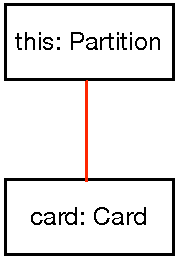
\includegraphics[width=0.2\textwidth]{goal_removeCard.pdf}
	\caption{Removing a card from its partition}
	\label{fig:goal_removeCard}
\end{figure}
\FloatBarrier

\vspace{0.5cm}

According to the signature of the method \texttt{removeCard}, we should return the card that has been deleted. Although this might strike you as slightly odd,
considering that we already passed in the card as an argument, it still makes sense as it allows for chaining method calls:
\syntax{ aPartition.removeCard(aCard).invert()}

Before we implement this change as a story diagram, let's remove the old injection content to avoid potential conflicts.

\begin{itemize}

\item[$\blacktriangleright$] Delete the \texttt{PartitionImpl.inject} file from your working set (Fig~\ref{eclipse:delete_injection}).

\item[$\blacktriangleright$] Now select \texttt{LearningBoxLanguage} and click on the ``Build" button. 

\item[$\blacktriangleright$] You'll be able to see the changes in \texttt{PartitionImpl.java}. The \texttt{removeCard}
declaration should now be empty and look identical to the other unimplemented methods.

\end{itemize}

\newpage

\begin{figure}[htbp]
	\centering
    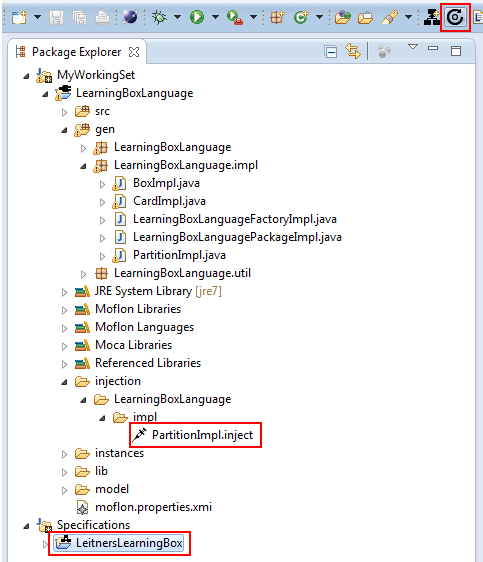
\includegraphics[width=0.5\textwidth]{eclipse_removeInjection}
	\caption{Remove injection content}
	\label{eclipse:delete_injection}
\end{figure}

\vspace{1cm}

That's it! We now have a fresh start for \texttt{removeCard}. Let's briefly discuss what we need to establish the transformation.

One of the goals of SDM is to allow you to focus less on \emph{how} a method will do something, but rather on \emph{what} the method will do.
Integrated as an atomic step in the overall control flow, a single graph transformation step (such as link deletion) can be embedded as a
\emph{story pattern}.

These patterns declare \emph{object variables}\define{Object \\ Variable}, place holders for actual objects in a model. During \emph{pattern matching}, objects
in the current model are assigned to the object variables in the pattern according to the indicated type and other conditions.\footnote{We shall learn what
further conditions may be specified in later SDMs.}

\clearpage

In \texttt{removeCard}, the SDM requires just two object variables: a \texttt{this} partition (named according to Java convention) referring to the
object whose method is invoked, and \texttt{card}, the parameter that will be removed.

Patterns also declare \emph{link variables}\define{Link \\ Variable} to match references in the model. Given that
we're concerned with removing a certain card from a specific partition, \texttt{removeCard} will therefore have a single link variable that connects these two
objects together.

In general, pattern matching is non-deterministic, i.e., variables in the pattern are bound to \emph{any} objects that happen to match. How can this
be influenced so that, as required for \texttt{removeCard}, the pattern matcher chooses the correct \texttt{card} (that which is passed in as a parameter)?

The \emph{binding state}\define{Binding~State} of an object variable determines how it is found. By default, every object variable is \emph{unbound}, or a 
\emph{free variable}\define{Free \\ Variable}. Values for these variables can be determined automatically by the pattern matcher. By declaring an
object variable that is to be \emph{bound}\define{Bound} however, it will have a fixed value determined from previous activity nodes. The appropriate binding is
implicitly determined via the \emph{name} of the bound object variable. As a rule, \texttt{this} variables, and any method parameters (i.e., \texttt{card}) are
always bound.

On a final note, every object or link variable can also set its \emph{binding operator} to \texttt{Check Only, Create, or Destroy}. For a rule $r: (L,
R)$, as discussed in \hyperlink{explanation}{Section 2}, this marks the variable as belonging to the set of elements to be retained ($L\cap R$), the set of
elements to be newly created ($R\setminus L$), or the set of elements to be deleted ($L\setminus R$).

If you're feeling overwhelmed by all the new terms and concepts, don't worry! We will define them again in the context of your chosen syntax with the
concrete example. For quick reference, we have also defined the most important terms at the end of this part in a \hyperlink{glossary}{glossary}. 

\jumpDual{remCard vis}{remCard tex}

\newpage
\hypertarget{remCard vis}{}
\subsection{Implementing removeCard}
\visHeader

\begin{itemize}

\item[$\blacktriangleright$] Re-open the LearningBoxLanguage diagram in Enterprise Architect (EA) from Eclipse by double-clicking the \texttt{.eap}
file. Carefully do the following: (1) Click \emph{once} on \texttt{Partition} to select it, then (2) Click \emph{once} on the method
\texttt{removeCard} to highlight it (Fig.~\ref{fig:sdm_start}), and (3) \emph{Double-click} on the chosen method to indicate that you want to implement it.

\begin{figure}[htp]
\begin{center}
  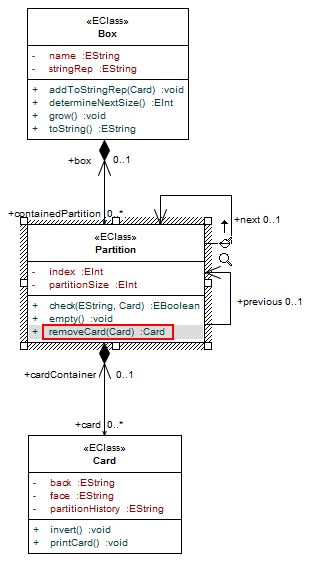
\includegraphics[width=0.6\textwidth]{ea_startSDM}
  \caption{Double-click a method to implement it}  
  \label{fig:sdm_start}
\end{center}
\end{figure}
 
\item[$\blacktriangleright$] If you did everything right, a new \emph{activity diagram} should be created and open in a new tab with a cute anchor in
the corner, and a \emph{start node} labelled with the signature of the method (Fig.~\ref{fig:sdm_skeleton}).  

\begin{figure}[htp]
\begin{center}
 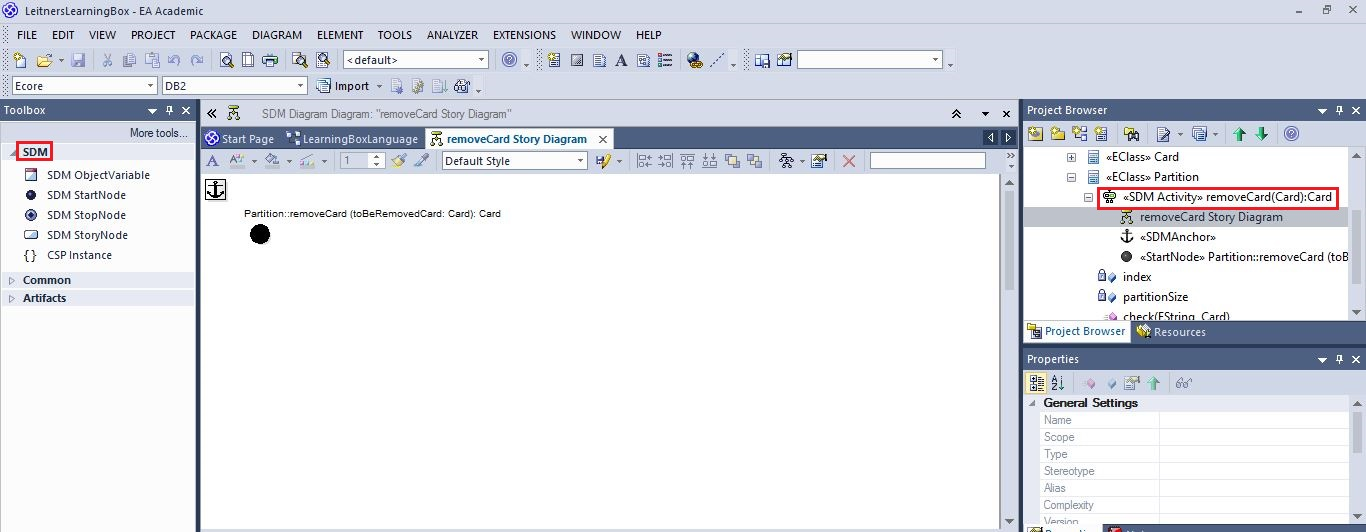
\includegraphics[width=1.0\textwidth]{ea_generatedSDM}
  \caption{Generated SDM diagram and start node}  
  \label{fig:sdm_skeleton}
\end{center}
\end{figure}

\vspace{0.5cm}

\item[$\blacktriangleright$] Let's quickly familiarise ourselves the EA workspace. First, inspect the project browser and notice that an \texttt{<<SDM
Activity>>} container has been created for the method \texttt{removeCard}. This container will eventually host every diagram related to this pattern. Please
note that, if you're at any time unhappy with an SDM,\footnote{As you might have already noticed, we use ``SDM'' interchangeably to mean our graph
transformation language \emph{or} a concrete transformation (a story model) used to implement a method and consisting of an activity diagram and a pattern in
each story node.} you can always delete the appropriate container in the project browser (such as this one), and start from scratch.

\vspace{0.5cm}

\item[$\blacktriangleright$] Next, note the new \texttt{SDM} toolbox that has been automatically opened for the diagram and placed to the left above
the common toolbox. This provides quick access to SDM items that you'll frequently use in your diagram.

\vspace{0.5cm}

\item[$\blacktriangleright$] Finally, in the top left corner of the diagram, you'll notice a small anchor. Double click on this icon to quickly jump back to the
metamodel. From there, double click the method again to jump back to the SDM. This is just a small trick to help you quickly shift between diagrams.

\vspace{0.5cm}

\item[$\blacktriangleright$] To begin, select the start node, and note the small black arrow that appears (Fig.~\ref{fig:sdm_quicklink}). 

\newpage

\begin{figure}[htp]
\begin{center}
  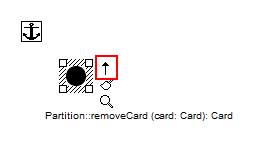
\includegraphics[width=0.5\textwidth]{ea_sdmStartNode}
  \caption{Quick link in SDM diagram to create new activity node}  
  \label{fig:sdm_quicklink}
\end{center}
\end{figure}

\item[$\blacktriangleright$] Similar to quick linking,\footnote{Learnt in Part II, Section 2.5} a second fundamental gesture in EA is \emph{Quick
Create}.
To quick-create an element, pull the arrow and click on an empty spot in the diagram. This is basically ``quick linking'' to a non-existent element.

\item[$\blacktriangleright$] EA notices that there is nothing to quick-link to, and pops a small context-sensitive dialogue to create an element that can be
connected to the indicated source element.

\item[$\blacktriangleright$] As illustrated in Fig.~\ref{fig:sdm_new_activity_node}, choose \texttt{Append StoryNode} to create an \emph{activity
node}. We refer to the whole activity diagram simply as the \emph{activity}, which always starts with a start node, terminates with a \emph{stop node}, and
consists of activity nodes connected via \emph{activity edges}.

\begin{figure}[htp]
\begin{center}
  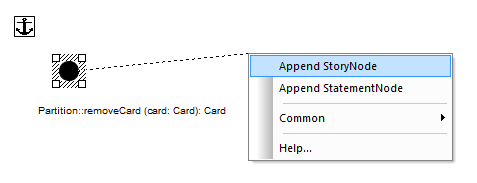
\includegraphics[width=0.8\textwidth]{ea_sdmQuickLinkStoryNode}
  \caption{Create new activity node}  
  \label{fig:sdm_new_activity_node}
\end{center}
\end{figure}

\item[$\blacktriangleright$] If you quick-created correctly, you should now have a start node, an activity node called \texttt{ActivityNode 1}, and an edge
connecting the two items. Complete the activity by quick creating a stop node as depicted in Fig.~\ref{fig:sdm_stop_node}.

\begin{figure}[htp]
\begin{center}
  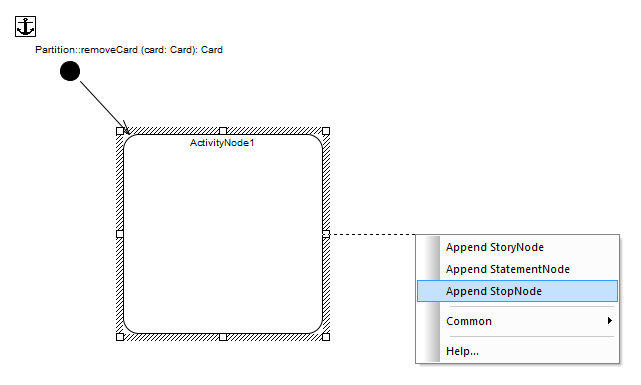
\includegraphics[width=\textwidth]{ea_sdmAppendStopNode}
  \caption{Complete activity with a stop node}  
  \label{fig:sdm_stop_node}
\end{center}
\end{figure}

\vspace{0.5cm}

\item[$\blacktriangleright$] If everything is correct, you should now have a complete activity that models the \emph{control flow} of the method. 
The semantics of our activity is pretty straightforward -- the control begins in the start node, and flows along edges and their connected activity nodes until
it reaches a stop node, where it finally terminates. 

\vspace{0.5cm}

\item[$\blacktriangleright$] While a \emph{stop node} is rather self explanatory, you may be wondering about the differences between the other two item options,
a\define{Story Node}\emph{story node}and a \emph{statement node}.\define{Statement Node}Since not all activity nodes can contain story patterns (i.e., start
and stop nodes), those that \emph{can} are called story nodes. Statement nodes are simply used to guarantee a certain action. They happen between story nodes.
We'll encounter these in a later SDM, but for now, lets finish our first story node.

\vspace{0.5cm}

\item[$\blacktriangleright$] To craft the story pattern, double click \texttt{ActivityNode 1} to prompt the dialogue depicted in
Fig.~\ref{fig:story_pattern}. Enter \texttt{removeCardFromPartition} as the name of the story node, and select \texttt{Create this Object}.  Click
\texttt{OK} - the activity node now has a single \emph{object variable}, \texttt{this} (Fig.~\ref{fig:tool_box}).

\begin{figure}[htpb]
\begin{center} 
  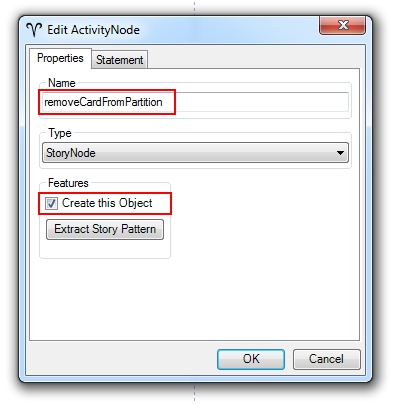
\includegraphics[width=0.6\textwidth]{ea_sdmEditActivityNode}
  \caption{Start modelling story pattern in activity node}  
  \label{fig:story_pattern}
\end{center}
\end{figure}

\begin{figure}[htp]
\begin{center}
  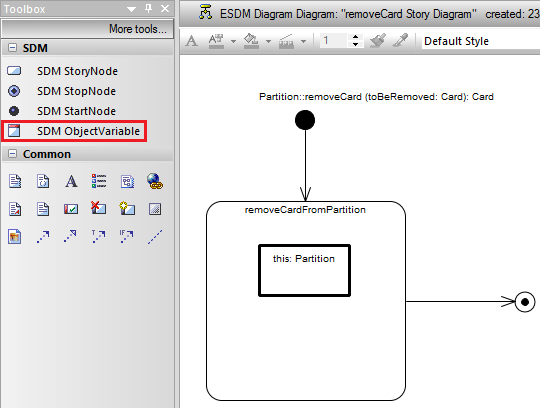
\includegraphics[width=0.8\textwidth]{ea_sdmNewObjVar}
  \caption{Add a new object variable from the toolbox}  
  \label{fig:tool_box}
\end{center}
\end{figure}

\newpage

\item[$\blacktriangleright$] To create an object variable that can be assigned to other objects, either choose \texttt{SDM ObjectVariable} from the toolbox or
press \texttt{ctrl}, then click inside the activity node (Fig.~\ref{fig:tool_box}). A properties window will be raised for the new object
(Fig.~\ref{fig:object_variable_properties}).

\vspace{0.5cm}

\begin{figure}[htp]
\begin{center}
  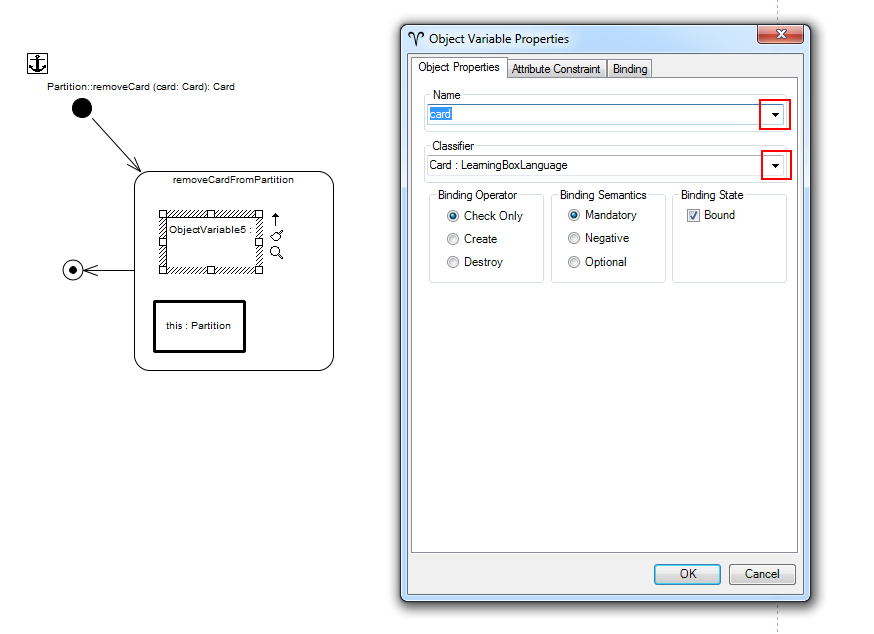
\includegraphics[width=\textwidth]{ea_sdmPropertiesObjVar}
  \caption{Specify properties of the added object variable}  
  \label{fig:object_variable_properties}
\end{center}
\end{figure}


\item[$\blacktriangleright$] Using the drop-down menus, choose \texttt{card} as the name of the object variable and set \texttt{Card} as its type.
Since \texttt{card} is a parameter of the method, it is offered as a possible name which can be directly chosen to prevent annoying typing mistakes.

\vspace{0.5cm}

\item[$\blacktriangleright$] In this dialogue, note that the \texttt{Bound} option must be set. We have now seen two cases in this activity for bound object
variables: an assignment to \texttt{this}, and an assignment to a method parameter. \texttt{Unbounded} object are represented by a thin-bordered box. Setting
\texttt{card} to bound means that it will implicitly assign itself to the passed parameter valued.

\item[$\blacktriangleright$] To create a \emph{link variable} between the current partition and the card to be removed, choose the object variable \texttt{this}
and quick-link it to \texttt{card} (Fig.~\ref{fig:link_variable}).

\begin{figure}[htpb]
\begin{center}
  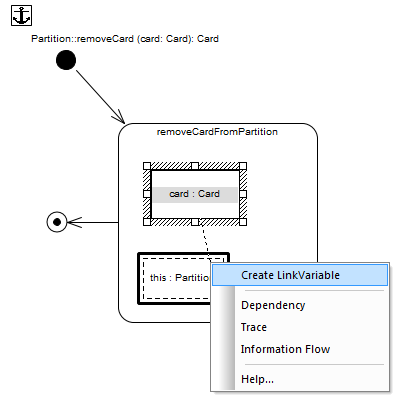
\includegraphics[width=0.6\textwidth]{ea_sdmCreateLinkVar}
  \caption{Create a link variable}   
  \label{fig:link_variable}
\end{center}
\end{figure}

\item[$\blacktriangleright$] According to the metamodel, there is only one possible link between a partition and card. Select this and set the
\emph{Binding Operator} to \texttt{Destroy} (Fig.~\ref{fig:link_variable_properties}). The reference names will automatically appear in the diagram.

\vspace{0.5cm}

% Had to force (h!) image to appear here; no other images were co-operating
\begin{figure}[h!]
\begin{center} 
 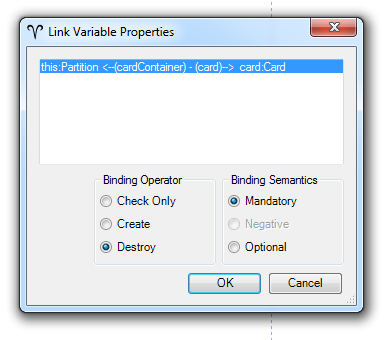
\includegraphics[width=0.6\textwidth]{ea_sdmBindLink}
  \caption{Specify properties for created link variable}  
  \label{fig:link_variable_properties}
\end{center}
\end{figure}

\vspace{0.5cm}

\item[$\blacktriangleright$] Remember how we said that this method should return the same card that was passed in? As luck would have it, a return value for any
SDM can be specified in the stop node. As depicted in Fig.~\ref{fig:stop_node_return_value}, double-click the stop node to prompt the \texttt{Edit StopNode} dialogue. 

\begin{figure}[htbp]
\begin{center}
  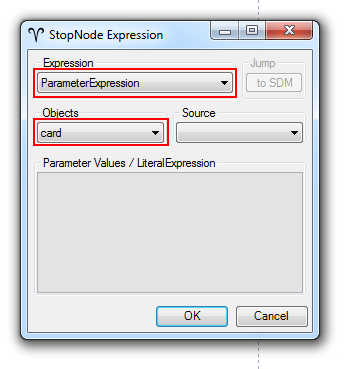
\includegraphics[width=0.5\textwidth]{ea_sdmStopNodeExpr}
  \caption{Adding a return value to the stop node}  
  \label{fig:stop_node_return_value}
\end{center}
\end{figure}

\item[$\blacktriangleright$] In the \texttt{Expression} field, choose \texttt{ParameterExpression}\define{ParameterExpression}as the expression. Given that
\texttt{card} is the sole parameter, it will be automatically selected. In EA, a \emph{ParameterExpression} is a mechanism that exclusively accesses any
paramter value.

\vspace{0.5cm}

We're nearly done! As you can see, by using several different dialouges, eMoflon employs a simple context-sensitive expression language for specifying required
values. We have intentionally avoided creating a full-blown sub-language, and limit expressions to a few simple types.\footnote{We also do not support nesting
expressions} The philosophy here is to keep things simple and concentrate on what SDMs are good for -- expressing structural changes. Our approach is to
provide a clear and type-safe interface to a general purpose language (Java) and support a simple \emph{fallback} as soon as things get too low-level and
difficult to express as a pattern.

The alternative approach to eMoflon would be to support arbitrary expressions, for example, in a script language like JavaScript or in an appropriate
DSL\footnote{A DSL is a Domain Specific Language: a language designed for a specific task which is usually simpler than a general purpose language like Java and
more suitable for the exact task.} designed for this purpose. In the following SDM implementations, we'll learn the other expression types eMoflon supports,
and how to use them. 

\item[$\blacktriangleright$] Returning to the activity, if you've done everything right, your first SDM completed with eMoflon should resemble
Fig.~\ref{fig:sdm_complete_control_flow}. The return value is indicated below the stop node.


\begin{figure}[htbp]
\begin{center}
  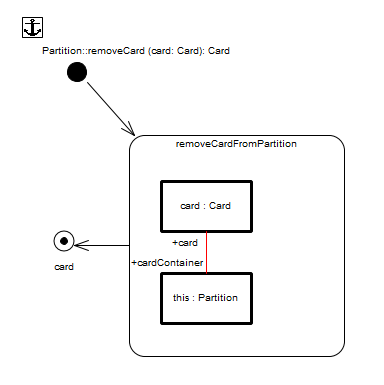
\includegraphics[width=0.7\textwidth]{ea_sdmRemoveComplete}
  \caption{Complete SDM for \texttt{Partition::removeCard}}  
  \label{fig:sdm_complete_control_flow}
\end{center}
\end{figure}

\item[$\blacktriangleright$]  Don't forget to save your files, validate and export your pattern to the Eclipse workspace,\footnote{Go to to
``\texttt{Extensions}" and select \texttt{Add-In Windows} to activate eMoflon's console. If you're unsure how to validate, export, or use this window, review
Part II, section 3} then build your metamodel's code from the package explorer.

\item[$\blacktriangleright$] If you're unable to export or generate code successfully, compare your SDM carefully with Fig.~\ref{fig:sdm_complete_control_flow}
and make sure you haven't forgotten anything.

\item[$\blacktriangleright$] If successful, navigate to ``Learning\-Box\-Language/\-gen/\-Learning\-Box\-Language/\-impl/\-Partition\-Impl.java" to the
\texttt{\-remove\-Card} declaration. Inspect the generated implementation for your method. Notice all the null checks that are automatically created - only a
very conscientious (and probably slightly paranoid) programmer would program so defensively!

Let's take a step back and briefly review what we have specified:  if \texttt{p.remove\-Card(c)} is invoked for a partition \texttt{p}, with a card, \texttt{c},
as its argument, the specified pattern will \emph{match} only if that card is contained in the partition. After determining matches for all variables, the
link between the partition and the card is deleted, effectively ``removing'' the card from the partition. If the card is \emph{not} contained in the partition,
the pattern won't match, and nothing will happen. In both cases, the card that's passed in is returned.

\item[$\blacktriangleright$] If you'd like to see how this SDM is implemented in the textual syntax, check out Fig.~\ref{fig:deleteReference} in the next
section.

\item[$\blacktriangleright$] Now we admit, this section had a lot of reading and theory, but it does get better. Soon, you'll be an eMoflon master, and we'll
hardly need to give you any instructions at all! In the following sections, we shall explore further features of SDM that allow for really expressive and
powerful patterns.

\fancyfoot[R]{ $\triangleright$ \hyperlink{sec:checkCard}{Next} }

\end{itemize}



\newpage
\hypertarget{remCard tex}{}
\subsection{Implementing removeCard}
\texHeader

\disclaimerForTextualSyntax

\begin{itemize}

\itemWithRightTriangle Open \texttt{Partition.eclass}, go to the
\texttt{removeCard} signature and add a pair of curly brackets so that it looks like a proper method declaration. This entire scope can be referred to as the method's \emph{activity}, where the control flow (imperative top-layer) of a
transformation is defined.

\itemWithRightTriangle Complete the activity with a single pattern and return statement as depicted in Fig~\ref{eclipse:remCardDec}. Don't forget -- you
can use eMoflon's auto-complete feature here! Press \texttt{Ctrl + Space} on an
empty line, then select the pattern template to establish \texttt{deleteSingleCard}.

\itemWithRightTriangle Note that in this context, the \texttt{`@'} operator indicates an \emph{ObjectVariableExpression}%
\define{ObjectVariable\-Expression}. This expression implicitly refers to object variables from the preceding story node. In \texttt{removeCard}'s case, the
returned object refers to the \texttt{card} from the pattern.

\vspace{0.5cm}

\begin{figure}[htp]
\begin{center}
  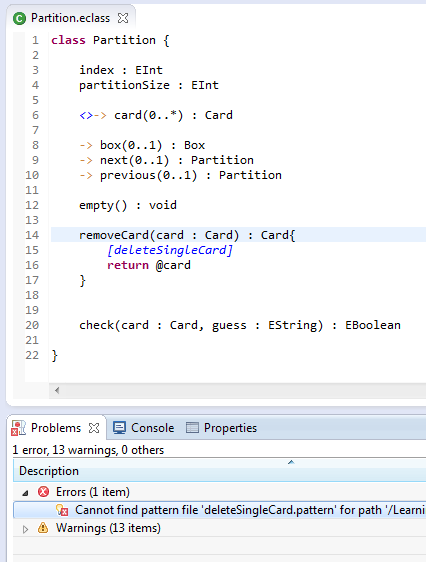
\includegraphics[width=0.5\textwidth]{eclipse_removeCardDeclaration}
  \caption{Control flow for \texttt{removeCard}}
  \label{eclipse:remCardDec}
\end{center}
\end{figure}

\itemWithRightTriangle It should be mentioned that MOSL limits method definitions exclusively to the method's control flow. All actual transformation
rules are modeled in separate \emph{pattern} files. In this case, \texttt{removeCard}'s link deletion will be modeled in \texttt{[deleteSingleCard]}.

\vspace{0.5cm}

\itemWithRightTriangle Save \texttt{Partition.eclass}. An error should immediately appear below the editor. In the ``Problems'' tab, the message
states that the builder cannot find the specified pattern file. Well, this makes sense. You haven't created it yet! Click this message and press \texttt{Ctrl +
1} to invoke a ``Quick Fix'' dialogue (Fig~\ref{eclipse:quickFix}). It offers to create a pattern file for you. Given that's exactly what you'd like, select the
option and press \texttt{Finish}.

\vspace{0.5cm}

\begin{figure}[htp]
\begin{center}
  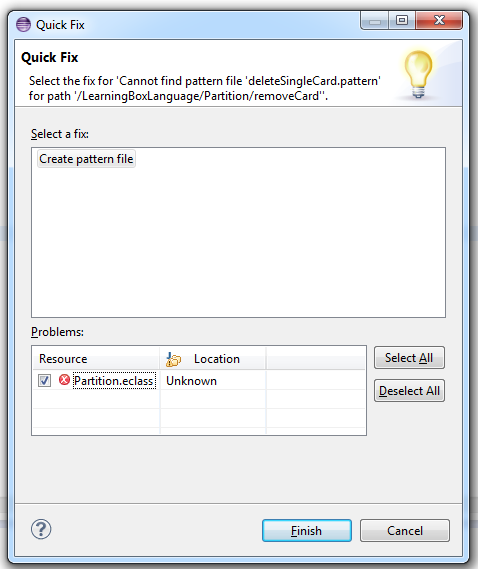
\includegraphics[width=0.5\textwidth]{eclipse_patternQuickFix}
  \caption{A quick fix to a missing pattern error}
  \label{eclipse:quickFix}
\end{center}
\end{figure}

\itemWithRightTriangle The new file will open in the editor, and you'll be able to see a new directory structure under ``LearningBoxLanguage/\_patterns''
(Fig.~\ref{eclipse:pattStruct}). To explain, \texttt{deleteSingleCard.pattern} is invoked by the method \texttt{removeCard}, which is in the \texttt{Partition}
EClass. \texttt{Partition} will eventually contain a folder for each method that uses a pattern.

\vspace{0.5cm}

\itemWithRightTriangle The content of any pattern file is simply a list \emph{object variable scopes}, and then,
within such a scope, operations such as `delete/create/find' this outgoing reference. Remember - the main goal of SDMs is to focus here is not on \emph{how},
but \emph{what}.

%\newpage

\begin{figure}[htp]
\begin{center}
  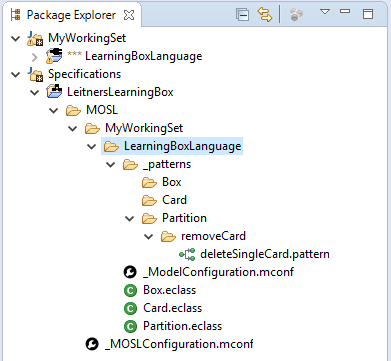
\includegraphics[width=0.9\textwidth]{eclipse_patternStructure}
  \caption{Directory structure for a pattern}
  \label{eclipse:pattStruct}
\end{center}
\end{figure}

\itemWithRightTriangle Create two object variables, \texttt{@this:Partition } and \texttt{ @card:Card}\\ (Fig.~\ref{eclipse:remCardObjVar}). When working
with MOSL patterns, \texttt{`@'} again indicates that the variable is \emph{bound}. \texttt{this} is bound to the object whose method is invoked,
while \texttt{card} is bound to the value of the parameter with the same name.

\begin{figure}[htp]
\begin{center}
  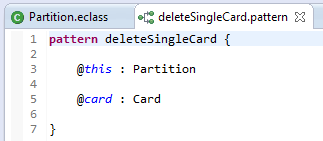
\includegraphics[width=0.6\textwidth]{eclipse_thisObjVar}
  \caption{Object variables for \texttt{removeCard}}
  \label{eclipse:remCardObjVar}
\end{center}
\end{figure}

\itemWithRightTriangle Object variable scopes determine the changes to be applied to the any exiting references of the variable. Therefore, add:
\syntax{-- -card-> card} to \texttt{@this} to destroy the \texttt{card} reference targeting the \texttt{card} object. Your pattern should now resemble
Fig.~\ref{eclipse:deleteReference}. 

\begin{figure}[htp]
\begin{center}
    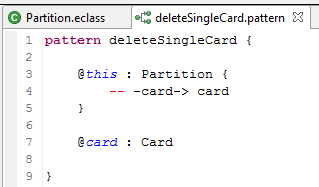
\includegraphics[width=0.6\textwidth]{eclipse_remCardObjVars}
  \caption{Destroy the link between a card and its partition}
  \label{eclipse:deleteReference}
\end{center}
\end{figure}
\newpage

\itemWithRightTriangle In summary, any \emph{outgoing link
 variable}\define{Outgoing~Link Var\-i\-able} follows this syntax:

\syntax{[action]`-'nameOfOutgoingLV`-> 'targetOV\\
\\
With:\\
action := `--' | `++' | `!'\\
nameOfOutgoingLV := STRING\\
targetOV := STRING
}

\itemWithRightTriangle If you ever need to quickly remind yourself of specific reference or attribute names, press \texttt{alt} and the \texttt{left}
arrow to jump back from your pattern to your EClass. Conversely, to quickly open
or jump to a pattern, hover over the pattern name while holding \texttt{Ctrl}
until it's underlined, then click!

\itemWithRightTriangle Remember, links between classes can be specified as \emph{bidrectional EReferences},\footnote{Technically two
\emph{unidirectional EReferences}. Refer to Part II, Section 2.5.} linked together as opposites in ``LearningBoxLanguage/\_con\-straints.mconf.'' In this case,
therefore, we don't need to worry about declaring \texttt{--
-cardContainer-> Card} inside \texttt{card}, as it would be redundant.

\itemWithRightTriangle Save and build your metamodel. If any errors occur, double check and make sure your activity and pattern match ours. 

\itemWithRightTriangle To see how the same method is crafted in the visual syntax, check out Fig.~\ref{ea:sdm_complete_control_flow} from the previous
section.

\end{itemize}


\newpage
\genHeader
\hypertarget{remCard end}{}
\subsubsection{Concluding removeCard}

Fantastic work! You have now implemented a simple method via patterns. As you can see, SDMs are effective for implementing structural changes in a high-level,
intuitive manner.

Let's take a step back and briefly review what we have specified:  if \texttt{p.remove\-Card(c)} is invoked for a partition \texttt{p}, with a card \texttt{c}
as its argument, the specified pattern will \emph{match} only if that card is contained in the partition. After determining matches for all variables, the
link between the partition and the card is deleted, effectively ``removing'' the card from the partition. If the card is \emph{not} contained in the partition,
the pattern won't match, and nothing will happen. In both cases, the card that's passed in is returned.

\begin{itemize}

\item[$\blacktriangleright$] If your code generation was successful, navigate to
``Learning\-Box\-Language/\-gen/\-Learning\-Box\-Language/\-impl/\-Partition\-Impl.java" to the \texttt{\-remove\-Card} declaration (approximately line 352).
Inspect the generated implementation for your method (Fig.~\ref{fig:remCardImpl}). Notice the null checks that is automatically created - only a very
conscientious (and probably slightly paranoid) programmer would program so defensively!

\vspace{0.5cm}

\begin{figure}[htp]
\begin{center}
  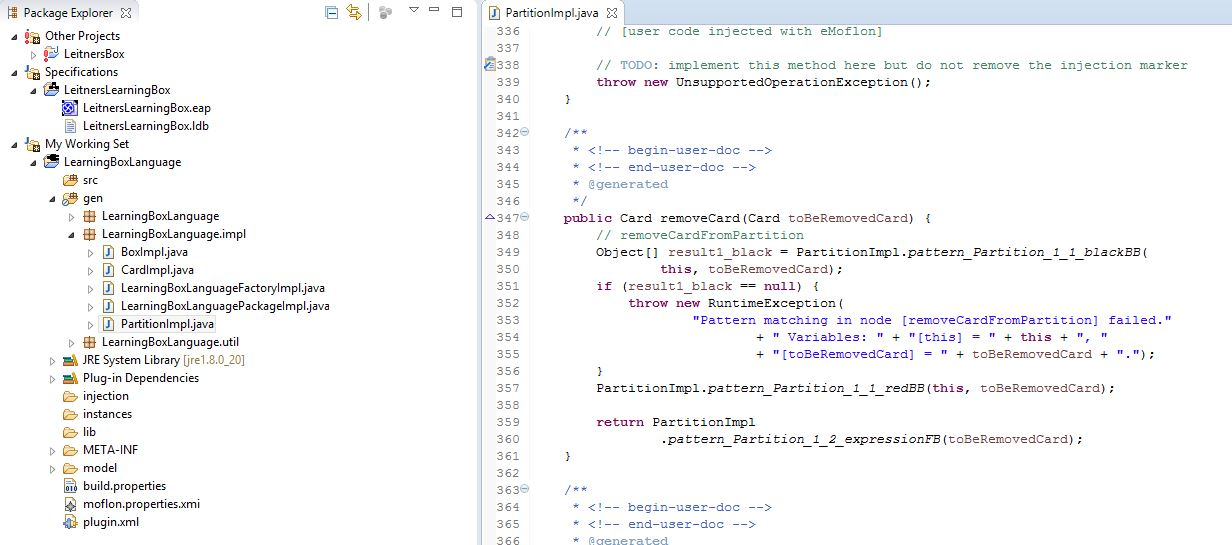
\includegraphics[width=\textwidth]{eclipse_remCardImpl}
  \caption{Generated implementation code}
  \label{fig:remCardImpl}
\end{center}
\end{figure}

\newpage

Near the end of Part II (after using injections), you were able to test this method's implementation using our \texttt{LeitnersBoxGui}. Let's run it again to
make sure \emph{this} version of \texttt{removeCard} works!

\item[$\blacktriangleright$] Load and run the GUI as an application,\footnote{Refer to Part II, Section 6 for details on our GUI} then go to any partition and
select \texttt{Remove Card} (Fig.~\ref{fig:GUIRemCard}).
It should immediately refresh, and you'll no longer be able to see the card in either the GUI or in the \texttt{Box.xmi} tree in the ``instances'' folder.
Pretty cool, eh?

\vspace{1cm}

\begin{figure}[htp]
\begin{center}
  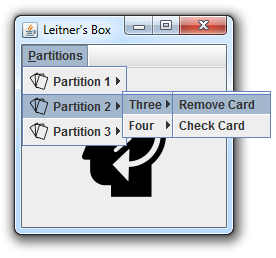
\includegraphics[width=0.5\textwidth]{eclipse_GUIRemove}
  \caption{Testing \texttt{removeCard}}
  \label{fig:GUIRemCard}
\end{center}
\end{figure}

\end{itemize}

